\documentclass{article}
\usepackage[utf8]{inputenc}
\usepackage{url,amsmath,graphicx,amssymb,booktabs,adjustbox,subcaption,hyperref,float}
\usepackage[top=1.5cm, bottom=1.5cm, left=2.5cm, right=2.5cm]{geometry}
\usepackage{tikz}
\usetikzlibrary{positioning,shapes.multipart}

\newtheorem{theorem}{Theorem}
\newtheorem{lemma}{Lemma}
\newtheorem{corollary}{Corollary}
\newtheorem{definition}{Definition}
\newtheorem{Proposition}{Proposition}

\newcommand{\Prob}{\mathbb{P}}
\newcommand{\E}{\mathbb{E}}
\newcommand{\Space}{\mathbb{S}}
\newcommand{\Var}{\text{Var}}
\newcommand{\MR}{\mathcal{R}}
\newcommand{\MT}{\mathcal{T}}

\title{MA3676 -  2018 Past Paper}
\author{1720996}

\begin{document}
\maketitle
\tableofcontents
\pagebreak

\section{Safe Answers}
\begin{table}[h]
    \centering
    \begin{tabular}{|c|c|c|c|c|}
        \hline
        Question & & & Marks & Total Question Marks\\
        \hline
        1 & a & i & $[1]$ &  \\
         & & ii & $[3]$ & \\
         & & iv & $[4]$ & \\
         & & v & $[1]$ & \\
         & & vi & $[6]$ & \\
         & b & & $[3]$ & $18/20$ \\
         \hline
        2 & a & & $[4]$ & \\
         & b & & $[6]$ & \\
         & c & & $[3]$ & \\
         & d & & $[7]$ & $20/20$ \\
        \hline
        3 & a & i & $[10]$ & \\
         & & ii & $[3]$ & $13/20$\\
        \hline
        Best Score & & & & $51/60=$ A+ \\
        \hline
    \end{tabular}
    \label{tab:safe}
\end{table}

\section{1}
\subsection{a}
\subsubsection{i}
\begin{equation}
    \mathbf{p} = \begin{pmatrix}
        0 & \frac{1}{2} & 0 & \frac{1}{2} & 0 & 0 & 0 \\
        0 & 0 & 0 & 0 & 0 & 1 & 0 \\
        0 & 0 & \frac{3}{4} & 0 & \frac{1}{4} & 0 & 0 \\
        \frac{1}{4} & 0 & \frac{1}{4} & \frac{1}{4} & 0 & 0 & \frac{1}{4} \\
        0 & 0 & \frac{1}{2} & 0 & \frac{1}{2} & 0 & 0 \\
        0 & \frac{1}{2}  & 0 & 0 & 0 & \frac{1}{2} & 0 \\
        0 & 0 & 0 & 0 & 0 & 0 & 1
    \end{pmatrix}.
\end{equation}

\subsubsection{ii}
\begin{figure}[H]
    \centering
    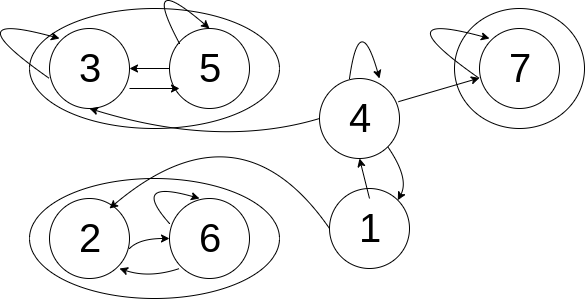
\includegraphics[scale=0.2]{diagram2018_1.png}
    \label{fig:1b}
\end{figure}
States $\{2,6\},\,\{3,5\},\,\{7\}$ are all closed recurrent sets of recurrent states, $1,4$ are transient.
\begin{equation}
    \mathbf{p} = \begin{pmatrix}
        0 & 1 & 0 & 0 & 0 & 0 & 0 \\
        \frac{1}{2} & \frac{1}{2} & 0 & 0 & 0 & 0 & 0 \\
        0 & 0 & \frac{3}{4} & \frac{1}{4} & 0 & 0 & 0 \\
        0 & 0 & \frac{1}{2} & \frac{1}{2} & 0 & 0 & 0 \\
        0 & 0 & 0 & 0 & 1 & 0 & 0 \\
        \frac{1}{2} & 0 & 0 & 0 & 0 & 0 & \frac{1}{2} \\
        0 & 0 & \frac{1}{4} & 0 & \frac{1}{4} & \frac{1}{4} & \frac{1}{4}
    \end{pmatrix}.\label{p_ii}
\end{equation}

\subsubsection{iii}
There are three closed sets of recurrent states, so three of the seven eigenvalues will be equal to one. The other four will have a magnitude less than one, with one of these being exactly equal to negative 1.

\subsubsection{iv}
Find the equilibrium state of the closed set by solving
\begin{equation}
    \begin{pmatrix}
    \pi_2 & \pi_6
    \end{pmatrix} = \begin{pmatrix}
    \pi_2 & \pi_6
    \end{pmatrix}\begin{pmatrix}
    0 & 1 \\ \frac{1}{2} & \frac{1}{2}
    \end{pmatrix},
\end{equation}
to give you 
\begin{equation}
    \pi_2 = \frac{1}{3} \quad \pi_6 = \frac{2}{3}.
\end{equation}
Therefore, our answer is $\pi_2 = \frac{1}{3}$. 

\subsubsection{v}
States $1,4$ are transient, so the answer is $0$.

\subsubsection{vi}
Using the matrix in (\ref{p_ii}), we derive
\begin{align}
    \mathbf{R} &= \left(\begin{array}{cc|cc|c}
         \frac{1}{2} & 0 & 0 & 0 & 0  \\
         0 & 0 & \frac{1}{4} & 0 & \frac{1}{4} 
    \end{array}\right),\\
    \mathbf{\tilde{R}} &= \begin{pmatrix}
    \frac{1}{2} & 0 & 0 \\
    0 & \frac{1}{4} & \frac{1}{4},\end{pmatrix}, \\
    \mathbf{Q} &= \begin{pmatrix}
    0 & \frac{1}{2} \\
    \frac{1}{4} & \frac{1}{4},
    \end{pmatrix}
\end{align}
and solve $\mathbf{\tilde{V}} = (\mathbb{I}-\mathbf{Q})^{-1}\mathbf{\tilde{R}}$ to find
\begin{equation}
    \mathbf{\tilde{V}} = \begin{pmatrix}
    \frac{3}{5} & \frac{1}{5} & \frac{1}{5} \\
    \frac{1}{5} & \frac{2}{5} & \frac{2}{5}
    \end{pmatrix}.
\end{equation}
\subsection{b}
The transition matrix can be written as
\begin{equation}
    \begin{pmatrix}
        a & b & 0 & 0 \\
        c & d & 0 & 0 \\
        e & 0 & f & 0 \\
        0 & 0 & g & 0 
    \end{pmatrix},\label{1_b}
\end{equation}
where the bottom-right $2x2$-matrix is $\mathbf{Q}$. We use this to solve 
\begin{align}
    \mathbf{\mu} &= (\mathbb{I} - \mathbf{Q})^{-1}\mathbf{e} \\
     &= \begin{pmatrix}
         1-f & 0 \\
         -g & 1
     \end{pmatrix}^{-1}\begin{pmatrix}
         1 \\ 1
     \end{pmatrix}\\
    &= \begin{pmatrix}
        \frac{1}{1-f} & 0 \\
        \frac{g}{1-f} & 1
    \end{pmatrix}\begin{pmatrix}
        1 \\ 1
    \end{pmatrix} \\
    &= \begin{pmatrix}
        \frac{1}{1-f} \\ 1+\frac{g}{1-f}     
    \end{pmatrix}= \begin{pmatrix}
        1.4 \\ 1.6
    \end{pmatrix}.
\end{align}
Solving this gives you the values of $f=\frac{2}{7}$ and $g=\frac{3}{7}$. Looking at the transition matrix back in (\ref{1_b}), we can see that $g$ must be equal to one, and therefore the information given in this question is not reliable.

\section{2}
\subsection{a}
The one-step transition matrix of the scenario is 
\begin{equation}
    \begin{pmatrix}
        0.8 & 0.2 & 0 & 0 \\
        0.05 & 0.75 & 0.2 & 0 \\
        0.05 & 0 & 0.75 & 0.2 \\
        0.1 & 0 & 0 & 0.9 
    \end{pmatrix}.\label{2a}
\end{equation}
It has an equilibrial solution because there are less than two closed sets.

\subsection{b}
Let $\mathbf{\pi}=(\pi_1,\,\pi_2,\,\pi_3,\,\pi_4)$ be our steady state of the transition matrix (\ref{2a}). We then solve
\begin{equation}
    \mathbf{\pi}\begin{pmatrix}
        0.8 & 0.2 & 0 & 0 \\
        0.05 & 0.75 & 0.2 & 0 \\
        0.05 & 0 & 0.75 & 0.2 \\
        0.1 & 0 & 0 & 0.9 
    \end{pmatrix} = \mathbf{\pi}.
\end{equation}
We obtain the linear equations:
\begin{align}
    0.8\pi_1 + 0.05\pi_2 + 0.05\pi_3 + 0.1\pi_4 &= \pi_1 \\
    0.2\pi_1 + 0.75\pi_2 &= \pi_2 \\
    0.2\pi_3 + 0.75\pi_3 &= \pi_3 \\
    0.2\pi_3 + 0.9\pi_4 &= \pi_4.
\end{align}
These can be solved in terms of $\pi_4$ to give
\begin{equation}
    \mathbf{\pi} = \left(\frac{25\pi_4}{32},\,\frac{5\pi_4}{8},\,\frac{\pi_4}{2},\,\pi_4\right) = \pi_4\left( \frac{25}{32},\,\frac{5}{8},\,\frac{1}{2},\,1 \right).
\end{equation}
Using the fact that the magnitude of $\mathbf{\pi}$ is one, we solve the following
\begin{equation}
    \pi_4\left( \frac{25 + 20 + 16 + 32}{32} \right) = 1,
\end{equation}
to find
\begin{equation}
    \pi_4 = \frac{32}{93}.
\end{equation}
This gives us the final equilibrium as
\begin{equation}
    \mathbf{\pi} = \left( \frac{25}{93},\,\frac{20}{93},\,\frac{16}{93},\,\frac{32}{93} \right),
\end{equation}
showing that the unemployment rate in the long run is $\pi_1 = \frac{25}{93}\approx 0.269\ldots$.

\subsection{c}
Using transition matrix (\ref{2a}), we note the in-goings and out-goings at each employment bracket, as well as the percentage of each that is taken into account.
\begin{table}[H]
    \centering
    \begin{tabular}{|c|c|c|c|}
    \hline
        Employment & Distribution & Salary & In/Outgoing \\
        \hline
        Unemployed & $25/93$ & $1500$ & $-100\%$ \\
        Level $1$ & $20/93$ & $2000$ & $+10\%$ \\
        Level $2$ & $16/93$ & $4000$ & $+10\%$ \\
        Level $3$ & $32/93$ & $6000$ & $+10\%$ \\
        \hline
    \end{tabular}
    \label{2c}
\end{table}
Expand this and calculate total monthly income $\mathbf{I}$:
\begin{align}
    \mathbf{I} &= -\left( \frac{25\mathbf{N}}{93}\times 1500\times 1 \right) + \left( \frac{20\mathbf{N}}{93}\times 2000\times 0.1 \right) + \left( \frac{16\mathbf{N}}{93}\times 4000\times 0.1 \right) + \left( \frac{32\mathbf{N}}{93}\times 6000\times 0.1 \right) \\
    &= \frac{\mathbf{N}}{93}\left[ -37500 + 4000 + 6400 + 19200 \right]\\
    &= -\frac{7900\mathbf{N}}{93}.
\end{align}
The country's treasury makes a loss of $-\frac{7900\mathbf{N}}{93}$ marks each month.

\subsection{d}
We create a new transition matrix such that
\begin{equation}
    \mathbf{p} = \begin{pmatrix}
        0.6 & 0.4 & 0 & 0 \\
        0.04 & 0.76 & 0.2 & 0 \\
        0.04 & 0 & 0.76 & 0.2 \\
        0.1 & 0 & 0 & 0.9 
    \end{pmatrix},
\end{equation}
alongside a new tax rate to derive the following:
\begin{table}[H]
    \centering
    \begin{tabular}{|c|c|c|c|}
    \hline
        Employment & Distribution & Salary & In/Outgoing \\
        \hline
        Unemployed & $0.146$ & $1500$ & $-100\%$ \\
        Level $1$ & $0.244$ & $2000$ & $+7\%$ \\
        Level $2$ & $0.203$ & $4000$ & $+7\%$ \\
        Level $3$ & $0.407$ & $6000$ & $+7\%$ \\
        \hline
    \end{tabular}
    \label{2d}
\end{table}
where our new distributions are found using the same method as that in question $2$b (use an online calculator, I use \url{http://psych.fullerton.edu/mbirnbaum/calculators/Markov_Calculator.htm}). We then go through the same process as $2$c to find our new income $\mathbf{I} = 42.94\mathbf{N}$ marks each month. This is definitely beneficial to the country's income.

\section{3}
\subsection{a}
\subsubsection{i}
Our first step decomposition is 
\begin{equation}
    g_n = \mathbb{E}[E_n\vert+1]\cdot \frac{2}{3} +  \mathbb{E}[E_n\vert+2]\cdot \frac{1}{3}.\label{3a_1}
\end{equation}
We then define the following:
\begin{align}
     \mathbb{E}[E_n\vert +1] = 1+g_{n+1},\\
      \mathbb{E}[E_n\vert+2] = 1+g_{n+2},
\end{align}
allowing us to rewrite (\ref{3a_1}) as
\begin{equation}
    g_n = 1 + \frac{2}{3}g_{n+1} + \frac{1}{3}g_{n+2}. \label{3a_2}
\end{equation}
As this walk terminates at both $k$ and $k+1$, the steps until termination at these positions is zero, hence
\begin{align}
    g_k = 0,\label{3a_b1}\\
    g_{k+1} = 0.\label{3a_b2}
\end{align}
These are our boundary conditions.\\
Lets get the solutions to the characteristic equation of (\ref{3a_2}):
\begin{align}
    1 &= \frac{2}{3}\lambda + \frac{1}{3}\lambda^2,\\
    3 &= 2\lambda+\lambda^2,\\
    0 &= \lambda^2+2\lambda-3,\\
    0 &= (\lambda-1)(\lambda+3),
\end{align}
Giving us roots of $\lambda=1,\,-3$. This means the solution to our inhomogeneous equation is given by
\begin{equation}
    g_n^{(general)} = A+B(-3)^n,
\end{equation}
where $-3$ is our $\lambda\neq 1$.\\
For the particular solution, we use a guess of $\alpha n^a$, where $a$ is the number of repeated roots ($1$, in our case) and substitute this into (\ref{3a_2}) is a \textit{function} of $n$.
\begin{equation}
    \alpha n = 1 + \frac{2}{3}\alpha(n+1) + \frac{1}{3}\alpha(n+2),
\end{equation}
solves to $\alpha = -\frac{3}{4}$ after making $n=0$ and simplifying. Therefore, the general solution is
\begin{equation}
    g_n = A + B(-3)^n - \frac{3}{4}n.
\end{equation}
We then use our boundaries from (\ref{3a_b1}) \& (\ref{3a_b2}) to set the following:
\begin{align}
    g_k &= A+B(-3)^k - \frac{3}{4}k = 0,\\
    g_{k+1} &= A+B(-3)^{k+1} - \frac{3}{4}(k+1) = 0.
\end{align}
Solving these simultaneously provides us with
\begin{align}
    A &= \frac{3}{4}k + 3,\\
    B &= \frac{3}{8}\left(-\frac{1}{3}\right)^{k}. 
\end{align}
Therefore, starting from $n=0$, the probability of termination is given by
\begin{equation}
    g_0 = A+B = \frac{3}{4}k+3+\frac{3}{8}\left( -\frac{1}{3} \right)^k.
\end{equation}

\subsubsection{ii}
$Y_n$ is martingale defined as $Y_n = S_n +\beta n$. For this to be true, the following equation must hold (and is subsequently solved)
\begin{align}
     \mathbb{E}[Y_{n+1}\vert\{S_i\}_{i=0}^n] &= Y_n = S_n+\beta n,\\
     &=  \mathbb{E}[(S_n+X_{n+1} + \beta(n+1)],\\
     &= S_n + \frac{4}{3} + \beta n + \beta = S_n+\beta n,\\
\end{align}
which is rearranged to show $\beta=-\frac{4}{3}$.\\
Note, $ \mathbb{E}[X] = \frac{4}{3}$ is shown true through
\begin{align}
     \mathbb{E}[X] = \mathbb{P}[X=1]\cdot  1 + \mathbb{P}[X=2] \cdot 2,\\
     &= \frac{2}{3}\cdot 1 + \frac{1}{3}\cdot 2 = \frac{4}{3}.
\end{align}
\subsubsection{iii}


\subsection{b}
\subsubsection{i}
\subsubsection{ii}

\section{4}
\subsection{a}
\subsection{b}
\subsection{c}
\subsection{d}
\subsection{e}
\subsection{f}
\subsection{g}





\end{document}
